%   % !TEX root = ../../VIII,3_Rahmen-TeX_9-0.tex
%  
%   Band VIII, 3 N.~?? 	Nachträge (VIII, 1)
%   Signatur/Tex-Datei:	LH_38_135
%   RK-Nr. 	55793
%				
%   Überschrift: 	An ex Sinclaro
%
%   edlabels:			6
%   Diagramme: 		1
%
%
\selectlanguage{ngerman}
\frenchspacing
%
\begin{ledgroupsized}[r]{120mm}
\footnotesize
\pstart
\noindent\textbf{Überlieferung:}
\pend
\end{ledgroupsized}
%
\begin{ledgroupsized}[r]{114mm}
\footnotesize
\pstart \parindent -6mm
\makebox[6mm][l]{\textit{L}}%
Auszüge mit Bemerkungen aus
\protect\index{Namensregister}{\textso{Sinclair} (Singlarius, Sinclarus), George gest. 1696}\textsc{G.~Sinclair},
\title{Ars nova et magna gravitatis et levitatis}, Rotterdam 1669\cite{00546}: 
LH~XXXVIII Bl.~135. 
Ein Blatt 4\textsuperscript{o};
oberer und linker Rand beschnitten.
Eine Seite auf Bl.~135~r\textsuperscript{o}, ein Absatz auf Bl.~135~v\textsuperscript{o}.
\pend
\end{ledgroupsized}
%
%
\vspace{5mm}
\begin{ledgroup}
\footnotesize
\pstart
\noindent%
\textbf{Datierungsgründe:}	
%
George Sinclairs\protect\index{Namensregister}{\textso{Sinclair} (Singlarius, Sinclarus), George gest. 1696}
%
\textit{Ars nova}\cite{00546} erschien 1669. 
%
Die Anschaffung eines Exemplars kann auf den 8.\ (18.) August 1670 datiert werden 
%
(\title{LSB} I, 2, S.~451). Bereits Anfang Oktober 1670 kennt Leibniz diese Veröffentlichung so gut, 
%
dass er sie mit anderen Büchern vergleichen kann (\title{LSB} II, 2, S.~106). 
%
Anfang 1671 exzerpiert er aus der \cite{00546}\textit{Ars nova} 
%
(\cite{02074}\textit{LSB} VI, 2 N.~43), darunter eine Stelle, die auch in den vorliegenden Auszügen vorkommt (S.~\refpassage{38_135_6a}{38_135_6b}).
%
Eine weitere Erwähnung des Autors in Zusammenhang mit Pendelaufhängungen ist auf Anfang 1672 datierbar (\cite{02075}\title{LSB} VIII, 1 N.~5, S. 63). 
%
Daraus ergibt sich ein Zeitraum für eine mögliche Abfassung.
\pend 
\end{ledgroup}
%
%
\selectlanguage{latin}
\frenchspacing
% \newpage%
\vspace{8mm}
\pstart%
\normalsize%
\noindent%
\lbrack135~r\textsuperscript{o}\rbrack\
\pend
%
\pstart
\centering
An ex 
%
\edtext{Sinclaro\protect\index{Namensregister}{\textso{Sinclair} (Singlarius, Sinclarus), George gest. 1696}}{\lemma{Sinclaro}\Cfootnote{\protect\index{Namensregister}{\textso{Sinclair} (Singlarius, Sinclarus), George gest. 1696}\textsc{G.~Sinclair}, \title{Ars nova et magna gravitatis et levitatis. Sive Dialogorum philosophicorum libri sex de aeris vera ac reali gravitate}, Rotterdam 1669\cite{00546}.}}
\pend
\vspace{\baselineskip}
%
\pstart\noindent
%
\hspace{1mm}\hspace{-1mm}% Trick, weil \edlabel nicht zu \par-Beginn sein darf
\edlabel{38_135_2a}%
\edtext{}{% 	%A-Fn
{\xxref%
{38_135_2a}{38_135_2b}}%
\lemma{\textit{Am Rand, gestrichen:}}%
\Afootnote{\footnotesize 
$\protect\begin{array}[t]{l}\phantom{3}300\\\phantom{3}4\\\overline{1200}\\\phantom{3}3\\\overline{3600}\\\phantom{3}2\\\overline{7200}\protect\end{array}$
\hspace{10mm}
$\protect\begin{array}[t]{r}1\\2\\3\\4\\5\\6\\\overline{21}\protect\end{array}$}}%
%
\edtext{}{% C-Footnote
{\xxref%
{38_135_2a}{38_135_3}}%
\lemma{Numerandae \lbrack...\rbrack\ vibrationum}%
\Cfootnote{%
\cite{00546}a.a.O., S.~556f.\ und 565f.}}%
% 
Numerandae sunt penduli\protect\index{Sachverzeichnis}{vibratio penduli}\protect\index{Sachverzeichnis}{pendulum} vibrationes 
%
\edtext{v.\,g.\ sint 6,}{\lemma{}\Bfootnote{v.\,g.\ sint \textit{(1)}~5 \textit{(2)}~6 \textit{erg~L}}}
%
\edtext{dividend\lbrack o\rbrack}{%
\lemma{}%
\Bfootnote{%
dividenda %
\textit{L ändert Hrsg.}%
}}
%
ita
%
\edtext{semidiameter in partes $1+2+3+4+5+6$}{\lemma{semidiameter}\Bfootnote{\textit{(1)}~ut \textit{(2)}~in partes \textit{(a)}~$1\smallfrown 2\smallfrown 3\smallfrown 4\smallfrown 5\smallfrown 6$ \textit{(b)}~$1+2+3+4+5+6$~\textit{L}}} 
%
seu 21.\edlabel{38_135_2b}
%
\edtext{Et summo intervallo tribuantur partes}{\lemma{Et}\Bfootnote{\textit{(1)}~summae tribuantur part \textit{(2)}~summo intervallo tribuantur partes~\textit{L}}}
%
6.\ sequenti 5.\ et ita porro. Ex his ducantur sinus ad quadrantem, et loca intersectionis erunt loca vibrationum.%
\edlabel{38_135_3}
%
\pend
\pstart
\edtext{Omnes vibrationes\protect\index{Sachverzeichnis}{vibrationes aequidiuturnae} sunt aequidiuturnae inter se et cum descensu perpendiculari.}{\lemma{Omnes\; \lbrack...\rbrack\ \;perpendiculari}\Cfootnote{\cite{00546}a.a.O., S.~566\textendash571.}} 
%
\edtext{%
Si primo minuto secundo absolvit 
%
\edlabel{38_135_5a}%
\edtext{}{% C-Footnote
{\xxref%
{38_135_5a}{38_135_5b}}%
\lemma{}%
\Afootnote{\textit{Unterhalb} ulnam inter descendendum: (At quid de ascensu?)}}%
ulnam inter 
%
\edtext{descendendum\edlabel{38_135_5b}, sequente}{\lemma{descendendum,}\Bfootnote{\textit{(1)}~post \textit{(2)}~sequente~\textit{L}}}
%
absolvet 3 ulnas.}{%
\lemma{Si primo\; \lbrack...\rbrack\ \;ulnas}%
\Cfootnote{%
\cite{00546}a.a.O., S.~573f.}}
%
\pend
%
\pstart%
%
%
\hspace{1mm}\hspace{-1mm}% Trick, weil \edlabel nicht zu \par-Beginn sein darf
\edlabel{38_135_4a}%
\edtext{}{% C-Footnote
{\xxref%
{38_135_4a}{38_135_4b}}%
\lemma{\textit{1.~Quo} \lbrack...\rbrack\ tempore}%
\Cfootnote{%
\cite{00546}a.a.O., S.~592f.}}%
\textit{1.~Quo longior funiculus,\protect\index{Sachverzeichnis}{funiculus} hoc plures vibrationes} in universum.
\pend
%
\pstart
\edtext{2.~Sed aequali temporis}{\lemma{2.~Sed}\Bfootnote{\textit{(1)}~eodem tempore \textit{(2)}~aequali temporis~\textit{L}}} 
%
differentia plures sunt vibrationes 
%
\edtext{\lbrack brevioris\rbrack.}{%
\lemma{}%
\Bfootnote{%
longioris %
\textit{L ändert Hrsg.\ nach Vorlage}%
}}
%
\edtext{Sed longioris}{\lemma{Sed}\Bfootnote{\textit{(1)}~longiores \textit{(2)}~longioris~\textit{L}}} 
%
vibrationes sunt diuturniores, \textit{modo idem sit pondus utrobique}.
\pend
%
\pstart
3.~\textit{Tertio pendulum\protect\index{Sachverzeichnis}{pendulum gravius} gravioris ponderis plures habet vibrationes, easque diutius perseverantes quam vibrationes penduli levioris\protect\index{Sachverzeichnis}{pendulum levius} ponderis, modo ambo sint aequalium longitudine funiculorum.}
\pend
%
\pstart
\textit{4.~Duo pendula aequalis ponderis at funiculorum longitudine inaequalium ut 2 ad 1.\ numero\protect\index{Sachverzeichnis}{numerus vibrationum} vibrationum differunt ut 3 ad 4.}
\pend 
%
\pstart
\textit{Nam} NB.\ \textit{assumtis duobus globulis ferreis, utrisque 28 unciarum, atque duobus funiculis,\protect\index{Sachverzeichnis}{funiculus} hoc pedum 9.\ illo} 
%
\edtext{\textit{$4 \frac{1}{2}$} invenit,}{%
\lemma{\textit{$4 \frac{1}{2}$}}%
\Bfootnote{%
\textit{(1)}~invenies, %
\textit{(2)}~invenit,~\textit{L}%
}}
%
\textit{pendulum longiori funiculo vibrationes dare 3.\ breviori 4.\ eadem temporis differentia}. Non exprimit, quot in universum. 
\pend 
%
\pstart
\rule{0pt}{24pt}%
$\left.\begin{array}{llllllll}
5.&\text{Cum ut}&3&\text{ad } 2.&\text{fuere ex longiore}&5.&\text{breviore}&6.\\
&\dotfill &8&\text{ad } 6&\dotfill &7.&\dotfill &8\\
&\dotfill &9&\text{ad } 7\frac{2}{10}&\dotfill &9&\dotfill &10
\end{array}\right\}$ vibrationes eodem tempore.%
\edlabel{38_135_4b}
%
\pend 
%
\pstart
%
NB.\ Qui hujus rationem reddiderit, item cur tot vibrationes in universum ex tanta longitudine et gravitate\lbrack,\rbrack\ magnum mysterium naturae detexerit.
\pend 
%
\pstart
\hspace{1mm}\hspace{-1mm}% Trick, weil \edlabel nicht zu \par-Beginn sein darf
%
\edlabel{38_135_6a}%
\edtext{}{% B-Footnote
{\xxref%
{38_135_6a}{38_135_6b}}%
\lemma{\textit{Tenui} \lbrack...\rbrack\ \textit{excurrat}}%
\Cfootnote{%
\cite{00546}a.a.O., S.~599.%
}}%
%
\textit{Tenui funiculo 37.\ digitos longo cum semisse annectatur globus ferreus}
%
\edtext{\lbrack\textit{28.}\rbrack}{%
\lemma{}%
\Bfootnote{%
38.\ %
\textit{L ändert Hrsg.\ nach Vorlage}%
}}
%
\textit{unciarum, ejus quaelibet simplex vibratio\protect\index{Sachverzeichnis}{vibratio} secundum horarium\protect\index{Sachverzeichnis}{secundum horarium} ad amussim dabit. Sed ut sint accurate, non ultra} 
%
\edtext{\lbrack\textit{30 vel}\rbrack}{%
\lemma{}%
\Bfootnote{%
\textit{30 vel} %
\textit{erg.\ Hrsg.\ nach Vorlage}%
}}
%
\textit{36 digitos globulos excurrat.}\edlabel{38_135_6b}%
\edtext{}{%
\lemma{\hspace*{1,6mm}%
\lbrack\textit{Fig.~1}\rbrack%
}\killnumber%
\Cfootnote{%
\cite{00546}a.a.O., S.~19. Leibnizens Angabe \glqq p.~18\grqq\ ändert Hrsg.}}
%
\pend 
%
%
\vspace{1.5em} %%%%%%%%% Diagramm 1
\centerline{%
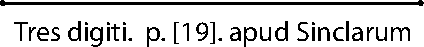
\includegraphics[width=0.4\textwidth]{%
gesamttex/edit_VIII,3/images/LH_38_135_d_135r.pdf%
}} 
\vspace{0.5em}
\centerline{%
\lbrack\textit{Fig.~1}\rbrack%
}
% \newpage%
\vspace{1.0em}
%
\pstart
\hspace{1mm}\hspace{-1mm}% Trick, weil \edlabel nicht zu \par-Beginn sein darf
%
\edlabel{38_135_1a}%
\textit{Appendatur}%
\edtext{}{% C-Footnote
{\xxref%
{38_135_1a}{38_135_1b}}%
\lemma{\textit{Appendatur} \lbrack...\rbrack\ \textit{nostratium}}%
\Cfootnote{%
\cite{00546}a.a.O., S.~607.}}
%
\textit{globulus ferreus duarum librarum funiculo cujusvis longitudinis, quem modo breviorem modo longiorem facies}\lbrack,\rbrack\ 
%
\textit{donec 16 exacte eveniant vibrationes, spatio}
%
\edtext{\textit{vig}\lbrack\textit{i}\rbrack\textit{nti}}{\lemma{}\Bfootnote{vigunti \textit{L ändert Hrsg.}}} 
%
\textit{secundorum, quibus factis, invenies funiculum} exacte \textit{aequare quantitatem septem pedum nostratium.}\edlabel{38_135_1b}
\pend
%
\pstart 
%
\lbrack135~v\textsuperscript{o}\rbrack\
%
\edtext{% C-Fn
Usus sum \textit{duobus} pendulis \textit{quorum} unum \textit{unciis pendebat octo, illud vero viginti octo, tamen nihil fere mutationis}
%
\edtext{\textit{a.}}{%
\lemma{\textit{a.}}%
\Cfootnote{\textit{aut}}}
%
\textit{discriminis inveni, nam ad unionem inter eorum vibrationes faciendam gravioris funiculum dimidium digiti solum, abbreviavi. Tardius ergo movetur pendulum grave}
%
\edtext{\textit{quam leve}}{\lemma{quam}\Bfootnote{\textit{(1)}~lege \textit{(2)}~leve~\textit{L}}}
%
\edtext{\textit{quatenus aer et medium pertranseundum magis ei obnititur.}}{\lemma{}\Afootnote{\textit{Am Rand}: NB}}}{%	C-Fn
\lemma{Usus \lbrack...\rbrack\ \textit{obnititur}}%
\Cfootnote{%
\cite{00546}a.a.O., S.~607 mit Auslassungen.}}
%
\pend 
\count\Afootins=1200%
\count\Bfootins=1200%
\count\Cfootins=1200